\chapter{Cetacean Detection Using Deep Learning}\label{ch:cetDet}

When building any large-scale project, it is important to break the task down into various subcomponents. In this Chapter we will examine one such subcomponent utilised in the developed automatic photo-id system, the cetacean detector. This component takes images captured during photo-id surveys and detects regions of interest, in our case these are dorsal fins which have breached the waterline. This Chapter will discuss the requirements a detector must meet, how it was trained, how the optimal hyperparameters were found, and how the detector can be utilised to provide a downstream identification system with only the information it needs. 

\section{Requirements of a Cetacean Detector}\label{ch:cetDet,sec:requirements}

Before a system for automatic cetacean detection can be developed, it is important to first define the problem and understand the requirements of the system. The overall aim of the detector is to be able to take large-scale images as input, fed in one at a time, and process them in order to locate regions of interest. Unlike other automated detection systems common in literature, this system is only required to detect one class of object, \texttt{dolphin}. These detected regions can then be passed further down the system pipeline to the identifier. 

 As such, this detector can be considered a coarse-grain task, and at first glance may seem somewhat trivial. However, due to both the nature of the environment in which the class must be detected, and the technical requirements the system must perform under, this becomes a much more complex problem. 
 
 \subsection{Environmental Requirements}\label{ch:cetDet,sec:requirements,sub:environmental}
 
 First the area in which this system is to be deployed, in open water, is susceptible to adverse weather conditions such as high winds. This in turn leads to sub-optimal conditions for detection which the system must be capable of handling, most notably high amounts of sea swell. Further to this, dolphins, the main data subject of this work, are communal and travel in pods. An example of this behaviour can be seen in Figure \ref{fig:pod-eg} Thus, the system must be capable of differentiating between overlapping individuals. Even if not all of the overlapping individuals are suitable for identification down the line, the system must still be able to separate them into individual detections to prevent further misclassification downstream; for example, lets assume an image is inputted to the detector containing three overlapping individuals where one of these has markings clear enough for a human to identify the individual. For our system to also be able to do this, the detector must be able to separate the overlapping animals into the individual components. This allows for the identifier to be provided with three images, one of which is the individual that is identifiable. If all overlapping individuals were passed to the identifier as one, the chance of identification will be greatly reduced, and the image may be identified as \texttt{noise}. 
 
 \begin{figure}
 	\begin{center}
 		\includegraphics[scale=0.06]{Chapter3/figs/dolphins-in-pod-example.JPG}
 	\end{center}
 	\caption{Some cetaceans, such as bottlenose dolphins, travel in pods. The developed detection system must be capable of splitting this pod into individual animals to be passed to the identifier.
 	}
 	\label{fig:pod-eg}
 \end{figure}

 Next, the detector must be capable of differentiating between dolphin fins and waves. Again this might sound trivial, but thousands of years of evolution have resulted in fins and waves looking extremely similar to the untrained eye, which artificial ones often start out as. Especially from a distance and in choppy waters, fins and waves often have extremely similar shape and dimensions. Furthermore, the animal's bodies are also similarly coloured to their surroundings. These adaptations allow the animals to be better protected and camouflaged in their environment, but can cause issues with detection systems. This becomes apparent when thinking about how CNNs \textit{see}. As described in Chapter \ref{ch:Background,sec:DLforCV}, CNNs see input images as a matrix of pixel values. When training an object detection system, the CNN is also told which parts of this matrix are related to a class, any without a class label are considered background. If fins and areas of background contain similar pixel values, and these pixel values are clustered in the same ways, this can result in issues when training a model to detect instances of a class without misclassifying the background. 
 
 Another important requirement is for the detector to be able to handle objects of varying size, shape, direction, and angle of approach to the camera. When working in an open water environment with live animals, the conditions that you will capture images of the animal under are extremely variable. You may capture an image of the animal at any point in it's breaching process, which will change the size of the dorsal fin which is above the waterline. As dorsal shape is unique to each individual, the detector must be capable of understanding a general `fin-shape' rather than a fixed one. 
 
  \begin{figure}
 	\begin{center}
 		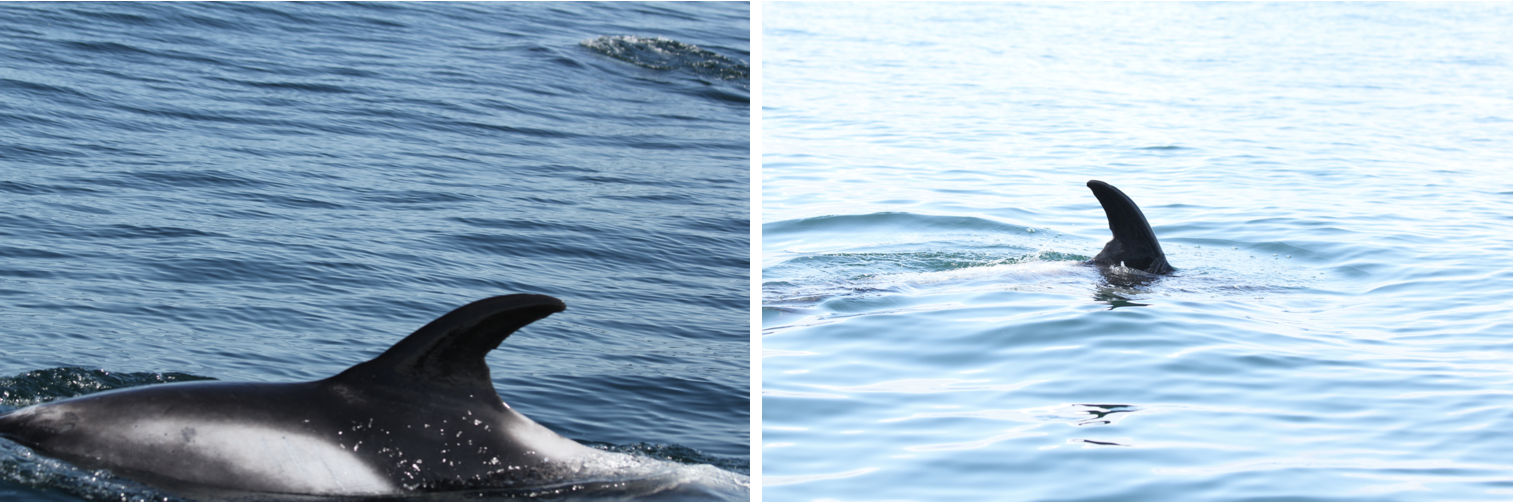
\includegraphics[scale=0.6]{Chapter3/figs/angle-size-example.png}
 	\end{center}
 	\caption{Two images of the same individual taken from different angles of approach, directions of travel, and distances from the vessel. Note how this changes the make-up of the dorsal fin, however keeps the identifying notch visible. 
 	}
 	\label{fig:angle-eg}
 \end{figure}
 
 Furthermore how the animals breach the waterline is also extremely variable. Breachings may occur at any  direction relative to the boat and the animal could itself be travelling in a different cardinality. The ideal scenario in this case would be for a breaching to occur either directly East or West of the boat (off the port or starboard side respectively) and for the animal to be travelling perpendicular as this provides the best chance of mark capture, however this rarely occurs. For example, a breaching may occur off the port-side of the bow (approx North West relative to the boat), but the animal may be travelling in a South-Easterly direction. These approaches greatly change the look of the fin, however they may still contain identifiable markings, thus our detector should be able to detect these fins and pass them along for identification. An example of this can be seen in Figure \ref{fig:angle-eg}, which also shows how distance from the vessel can change the camera's view of the dorsal. 
 
 As mentioned previously, weather conditions can also greatly affect how a dorsal fin is captured by a camera. However, especially in mark-recapture surveys, there are only two conditions that need to be worried about; swell and lighting, other conditions do not need to be handled by this detector. This is due to most research groups having limits of sea state for safety reasons. With regards to Newcastle University's Marine MEGAfauna Lab, this limit is a sea state less than 3 on the Beaufort scale \cite{world_meteorologicial_society_beaufort_1970}. As such a mild amount of swell and splash can be expected, which the detector should be capable of handling. Lighting conditions are not considered in the Beaufort scale, but for operational reasons the vast majority of mark-capture surveys take place during daylight hours. This can lead to large amounts of glare in images, especially on clear days. As such, the detector should be invariant to these conditions. 
 
 \subsection{Technical Requirements}\label{ch:cetDet,sec:requirements,sub:technical}
 
 As well as being able to handle a variety of environmental factors, there are also some technical requirements that the detector must meet. With all deep learning based computer vision approaches, there is often a trade off that must be made between speed and accuracy. In most cases, these are inversely proportional to each other; the faster a system is required to perform, the lower an accuracy you must be willing to tolerate - Huang \textit{et al.} discuss this in greater detail in their 2017 paper \cite{huang_speedaccuracy_2017}. Thanks to the pace of research in this area, 2020 saw the release of object detection architectures which can perform operations in real-time such as EfficientDet \cite{tan_efficientdet_2020} and YOLOv4 \cite{bochkovskiy_yolov4_2020}. Current results on benchmark datasets using these real-time architectures are still a long way off their non-real-time competitors however, and accuracies would drop further on custom non-benchmark tasks such as cetacean detection. 
 
 Because this trade off must be made, before deploying a deep learning model it is important to decide where the system will be utilised. As photo-id surveys are performed on small vessels such as RIBs, space is severely limited on board. Because of this, it is not appropriate to add additional hardware to the vessel to perform this analysis during the survey. Furthermore, the current methodology of cetacean researchers is to perform identification once back on land, even when utilising photo-id aides. As the system proposed in this project is intended to fit into existing procedures rather than replace researchers, it is appropriate for the system to also be land based rather than on the vessel. Thinking about the current procedure further, this project's proposed system could be, for example, left running overnight performing identifications whilst the researchers are away or during the day whilst they are on surveys, being left to work through the last day's worth of images captured. As such, there is no need for the system to operate in real time to fit in with the current workflow of cetacean researchers, provided the system completes its task within a reasonable time frame. Further to this, as the output of the detection model will be passed to an identification module, it is imperative that as much noise is removed as possible during the detection. In order to do this, the accuracy of the detection must be as high as possible, furthering the case for an accurate system over a fast one.
 
 This idea of reducing as much noise as possible can be used to further narrow down the requirements of the detection system. As discussed in Section \ref{ch:Background,sec:DLforCV}, the output of detection systems can be provided in different formats. In bounding box detection systems the detected objects are denoted by a set of at least two pixel coordinates denoting the top-left and bottom-right extremes of the object. These detections are often more cost-effective to perform computationally, however as we will only know the area of the image a detected object is present in, this does not remove all of the background noise, only that which is outside of the object's extreme points. If we utilise pixel wise mappings however, then each pixel is given a classification. This allows the system to be more discrete with its detection, telling us exactly where the object is in the image. These pixel locations can then be used to removed all background. As such, the use of pixel-wise mappings is more appropriate for our detector to use. Both semantic and instance segmentation methods will allow the detector to utilise pixel-wise mappings to remove background noise. However, utilising our requirement defined earlier in Section \ref{ch:cetDet,sec:requirements,sub:environmental} that the detector must be capable of reducing an overlapping pod to its individual component animals, it makes sense to require the detector to utilise instance segmentation.
 
\section{Deciding on Architecture and Framework}\label{ch:cetDet,sec:deciding}

Based on the requirements outlined in Section \ref{ch:cetDet,sec:requirements}, it is possible to begin deciding on how the cetacean detector is to be developed. One of the major decisions that must be made here is which model architecture should be utilised in order to provide the required pixel-level detections. As this project is devoted to improving existing procedures and introducing deep learning to a novel space, it is far more advantageous to utilise existing model architectures rather than develop a custom one. The development of a custom architecture for this stage of the project would be extremely time consuming, taking away time from more novel parts of the project (notably the identification of the individual animals). Further, as this project is introducing deep learning methods to a novel space, the project needs to be able to convince researchers in this space that the system is reliable; this is more easily achieved using a pre-existing architecture where use cases already exist in literature and business. 

To this end there are two main model architectures that can be chosen for this task; U-Net \cite{ronneberger_u-net_2015} and Mask-RCNN \cite{he_mask_2017}. Both of these architectures work in different ways. Vuola \textit{et al.} provide a more detailed comparison between the two models \cite{vuola_mask-rcnn_2019}, however the main focus for this project is their resultant output mask structure. 

U-Net is based on an encoder-decoder architecture. This allows for fast and simple segmentation when working with images where you only require one output. For example, taking U-Net's original use case of biomedical imaging, let's assume we have an image showing a group of cells and we wish to segment them into the individual components. U-Net is able to perform this operation efficiently through boundary estimation to locate the outer edges of the cells which allows them to be segmented from each other. However this results in an output of the same dimensions as the input, that is, all segmentations are provided in a single binary mask. 

In contrast, Mask-RCNN utilises a multi-stage architecture (described in more detail in Section \ref{ch:Background,sec:instanceSegmentation,sub:Mask R-CNN}). This allows the architecture to place each detection on its own binary output mask. This is extremely important for our use case; as our detector will be used as part of a larger system, passing information downstream to the identifier which will require individuals to be in their own images, processing each individual in series. If U-Net was utilised for the detection stage, whilst initially being more efficient than Mask-RCNN, further processing of the binary output mask would be required to split this into it's individual components. In contrast, if Mask-RCNN was utilised then the processing required in between the detection and identification stage would be far simpler. Again, this allows for more time to be spent working on the novel aspects of this project whilst keeping the pipeline as simple as possible. This reason was a big factor in deciding to focus on Mask-RCNN for this stage.

Another factor which must be decided upon when starting developing a deep learning system is the language and framework to be used for development. With regards to language this was a fairly simple decision; the vast majority of deep learning research and development is written in Python. The language benefits from an efficient and lightweight syntax as well as having a host of different deep learning packages available to aid in development. Further to this, both of the major deep learning frameworks, Google's Tensorflow \cite{abadi_tensorflow:_2016} and Facebook's Torch (of which PyTorch is the most actively developed) \cite{paszke_automatic_2017}, both provide full Python support and have active communities for the language. Thanks to this, the vast majority of deep learning development is performed using Python in one of these two frameworks. By utilising these technologies, this project's code is easily reproducible and understood, as well as extendable in the future.

Of the two main frameworks, the use of Tensorflow was decided for this project. Whilst this decision was made somewhat due to personal preference, Tensorflow was (at least at the time of starting this project) the primary framework for development of deep learning systems outside of academia. Rather than developing a custom Mask-RCNN in Tensorflow for this project, Matterport's Mask R-CNN implementation \cite{waleed_mask_2017} has been adapted. Whilst this implementation does require the use of an old version of Tensorflow (1.14), this version is also stable unlike the most recent versions (>= 2.0).


%%%%%%%%%%%%%%%%%%%
\nomenclature[z-CNN]{CNN}{Convolutional Neural Networks}
\nomenclature[z-CV]{CV}{Computer Vision}
\nomenclature[z-CPU]{CPU}{Central Processing Unit}
\nomenclature[z-GPU]{GPU}{Graphical Processing Unit}
\nomenclature[z-SGD]{SGD}{Stochastic Gradient Descent}
\nomenclature[z-ReLU]{ReLU}{Rectified Linear Unit}
\nomenclature[z-FCN]{FCN}{Fully Convolutional Network}
\nomenclature[z-RPN]{RPN}{Region Proposal Network}
